 \iffalse
\let\negmedspace\undefined
\let\negthickspace\undefined
\documentclass[journal,12pt,twocolumn]{IEEEtran}
\usepackage{cite}
\usepackage{amsmath,amssymb,amsfonts,amsthm}
\usepackage{algorithmic}
\usepackage{graphicx}
\usepackage{textcomp}
\usepackage{xcolor}
\usepackage{txfonts}
\usepackage{listings}
\usepackage{enumitem}
\usepackage{mathtools}
\usepackage{gensymb}
\usepackage{comment}
\usepackage[breaklinks=true]{hyperref}
\usepackage{tkz-euclide} 
\usepackage{listings}
\usepackage{gvv}                                        
\def\inputGnumericTable{}                                 
\usepackage[latin1]{inputenc}                                
\usepackage{color}                                            
\usepackage{array}                                            
\usepackage{longtable}                                       
\usepackage{calc}                                             
\usepackage{multirow}                                         
\usepackage{hhline}                                           
\usepackage{ifthen}                                           
\usepackage{lscape}
\usepackage{caption}
\newtheorem{theorem}{Theorem}[section]
\newtheorem{problem}{Problem}
\newtheorem{proposition}{Proposition}[section]
\newtheorem{lemma}{Lemma}[section]
\newtheorem{corollary}[theorem]{Corollary}
\newtheorem{example}{Example}[section]
\newtheorem{definition}[problem]{Definition}
\newcommand{\BEQA}{\begin{eqnarray}}
\newcommand{\EEQA}{\end{eqnarray}}
\newcommand{\define}{\stackrel{\triangle}{=}}
\theoremstyle{remark}
\newtheorem{rem}{Remark}
\begin{document}
\parindent 0px
\bibliographystyle{IEEEtran}
\vspace{3cm}

\title{NCERT 11.9.3 28Q}
\author{EE23BTECH11012 - Chavan Dinesh$^{*}$% <-this % stops a space
}
\maketitle
\newpage
\bigskip

\renewcommand{\thefigure}{\arabic{figure}}
\renewcommand{\thetable}{\arabic{table}}
\large\textbf{\textsl{Question:}}
The sum of two numbers is $6$ times their geometric mean, show that numbers are in the ratio $\dfrac{(3+2\sqrt{2})}{(3-2\sqrt{2})}$.

\solution
\fi
Let the two numbers be $x(0)$ and $x(2)$ such that $x(2)\geq x(0)$ 
% and $x(1)$ is G.M of $x(0)$ and $x(2)$.
\begin{table}[htbp]
    \centering
     \begin{tabular}{|c|c|c|}
        \hline
        \textbf{Parameter} & \textbf{Description} &\textbf{Value}\\
        \hline
        $x(0)$ & first number& \\
         \hline
        $r$ & common ratio &\\
        \hline
        $x(2)$ & second number & $x(0)r^2$\\
        \hline
        $x(1)$ & G.M & $x(0)r$\\
        \hline
        $x(n)$ & $(n + 1)^{th}$term & $(x(0)r^n)u(n)$\\
        \hline
    \end{tabular}
 

    \caption{Input table}
    \label{tab:parameter_table.11.9.3.28}
\end{table}

From \tabref{tab:parameter_table.11.9.3.28}:
\begin{align}
x(0) + x(2) &= 6x(1) \\
\implies x(0) + x(0)r^2 &= 6x(0)r \\
\implies r^2 - 6r +1 &= 0 \\
\implies r &= 3\pm 2\sqrt{2}\\
% \end{align}
% \begin{align}
    \therefore \frac{x(2)}{x(0)} &= (3 + 2\sqrt{2})^2 \\
    &=  \frac{(3+2\sqrt{2})}{(3-2\sqrt{2})}
\end{align}
\begin{align}
x(n) = (x(0)(3 + 2\sqrt{2})^n)u(n)
\end{align}
Taking z - Transform of $x(n)$:
\begin{align}
    X(z) = \frac{x(0)}{1 - (3 + 2\sqrt{2})z^{-1}} ; |z| > (3 + 2\sqrt{2})
\end{align}
\begin{figure}[ht]
    \centering
    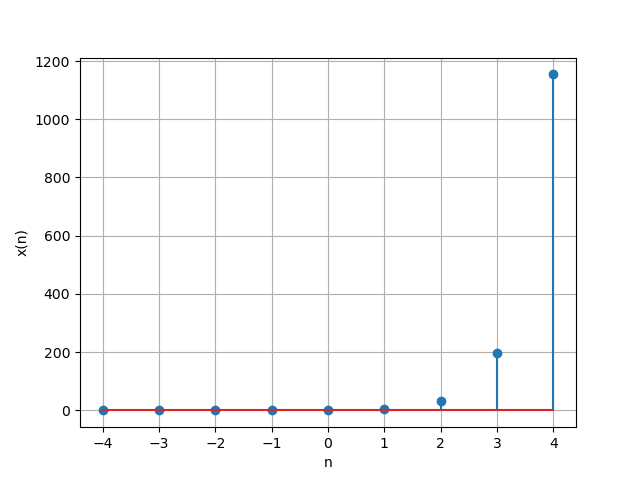
\includegraphics[width = \columnwidth]{ncert-maths/11/9/3/28/figs/x_n_stem_plot.png}
    \caption{}
    \label{fig:graph1.11.9.3.28}
\end{figure}

\bibliographystyle{IEEEtran}
